\documentclass[11pt,a4paper]{article}

\usepackage[margin=2.4cm]{geometry}
\usepackage{graphicx}
\usepackage{booktabs}
\usepackage{longtable}
\usepackage{array}
\usepackage{caption}
\usepackage{subcaption}
\usepackage{float}
\usepackage{hyperref}
\usepackage{xcolor}

\hypersetup{
    colorlinks=true,
    linkcolor=blue,
    urlcolor=blue,
    citecolor=blue
}

\captionsetup{font=small, labelfont=bf}
\renewcommand{\arraystretch}{1.15}
\newcommand{\code}[1]{\texttt{\detokenize{#1}}}
\newcommand{\metricci}[3]{#1 (#2-#3)}

\title{Technical Methodology\\
\large Interpretable Machine Learning for Predicting Surgical Risk in Skull-Base Meningioma}
\date{}

\begin{document}
\maketitle

\section{Aim and objectives}

We aimed to develop and evaluate supervised machine-learning models for predicting adverse postoperative outcomes after Skull-Base Meningioma (SBM) surgery using variables that are available before surgery. In practical terms, we asked the following question: given a patient's baseline clinical characteristics and radiological tumor features, can a statistical model estimate the probability of relevant postoperative risk before the operation?

We defined the following technical objectives:

\begin{enumerate}
    \item to implement a reproducible modeling workflow for heterogeneous clinical tabular data;
    \item to compare several machine-learning model families rather than relying on a single algorithm;
    \item to tune hyperparameters using a temporally ordered validation design, so that model selection is based on later cases than those used for fitting;
    \item to evaluate final models on a held-out temporal test set that is not used for fitting or hyperparameter selection;
    \item to select clinically conservative binary decision thresholds, with special attention to recall because false-negative predictions may be undesirable in surgical-risk screening;
    \item to quantify variable contribution by permutation feature importance; and
    \item to study whether a reduced list of input variables can preserve most predictive performance while making future doctor-facing prediction more practical.
\end{enumerate}

This last point is important for clinical usability. A model that requires a clinician to manually enter approximately 40 fields for each patient is unlikely to be used consistently in practice. We therefore used feature-importance analysis not only for interpretation, but also as an engineering tool for reducing the data-entry burden and limiting redundant predictors. Redundancy reduction may also improve generalization, since correlated or weakly informative variables can increase variance and encourage models to fit accidental patterns in a retrospective dataset.

\section{Machine-learning models}

Before introducing the dataset and experiments, we briefly describe the model families used in the study. All models receive the same preoperative patient variables, but they differ in how they learn relationships between predictors and postoperative outcomes. We compared five binary classifiers: histogram gradient boosting, random forest, logistic regression, support vector classifier, and multilayer perceptron. The classical scikit-learn models were implemented through scikit-learn, and the neural-network model was implemented with PyTorch \cite{pedregosa2011scikit,paszke2019pytorch}.

\subsection{Histogram gradient boosting}

Histogram Gradient Boosting (HGB) is an ensemble of decision trees built sequentially. Each new tree is trained to improve the errors made by the previous ensemble, following the general gradient-boosting principle \cite{friedman2001gradientboosting}. Continuous variables are internally grouped into bins, which makes training efficient on tabular data. This model can represent nonlinear effects and interactions, such as a different effect of tumor size depending on vascular involvement. Its main hyperparameters are the learning rate, number of boosting iterations, maximum tree depth, and L2 regularization. Class imbalance was addressed by giving higher fitting weight to minority-class observations.

\subsection{Random forest}

Random Forest (RF) is an ensemble of decision trees trained with random variation in the sampled patients and candidate split variables \cite{breiman2001randomforests}. Each tree produces a prediction, and the forest averages these predictions. This reduces the instability of a single decision tree and is often effective for clinical tabular data because it captures nonlinearities and interactions without assuming a linear relationship. Important hyperparameters include the number of trees, maximum tree depth, minimum samples per leaf, and the number of candidate features considered at each split. Class imbalance was handled through balanced class weights.

\subsection{Logistic regression}

Logistic Regression (LR) is a classical baseline for binary clinical prediction \cite{cox1958binary}. It models the log odds of the outcome as a weighted sum of predictors. Because it assumes an approximately linear relationship between predictors and log odds, it is less flexible than tree ensembles or neural networks, but it is stable and comparatively interpretable. We standardized numeric predictors for logistic regression because coefficient estimation depends on variable scale. The main tuning parameter is \code{C}, the inverse strength of regularization; smaller values impose stronger shrinkage and can reduce overfitting when the number of predictors is large relative to the number of events. We evaluated \code{lbfgs} and \code{liblinear} solvers and used balanced class weights for imbalanced endpoints.

\subsection{Support vector classifier}

The Support Vector Classifier (SVC) finds a decision boundary that separates classes with the largest possible margin \cite{cortes1995support}. With a linear kernel it behaves like a margin-based linear classifier, whereas with a radial-basis-function kernel it can learn nonlinear boundaries. We standardized numeric predictors because support vector classifiers are sensitive to feature scale. We enabled probability estimation so that AUROC, precision-recall curves, and threshold selection could be computed. The main hyperparameters are \code{C}, kernel type, and \code{gamma}, which controls how local the nonlinear decision boundary is. Class imbalance was handled through balanced class weights.

\subsection{Multilayer perceptron}

The MultiLayer Perceptron (MLP) is a feed-forward neural network implemented in PyTorch and wrapped as a scikit-learn-compatible estimator. It receives the tabular feature matrix and passes it through hidden layers with nonlinear activation functions, optional dropout, and a final binary output layer. This model family is based on layered nonlinear transformations trained by back-propagation \cite{rumelhart1986backpropagation}. We standardized numeric predictors because neural-network optimization is sensitive to feature scale. For binary endpoints, the network uses a sigmoid output and binary cross-entropy loss. Class imbalance was handled by weighting the positive class in the loss function. The main hyperparameters are hidden-layer size, dropout, learning rate, weight decay, batch size, and number of epochs.

\section{Data source, endpoints, and modeling population}

\subsection{Dataset and raw data structure}

For the analysis, we employed a dataset provided by ... (Noa, I don't have much information for this point), which contains a total of 731 rows (i.e. \emph{datapoints}) and 100 columns (i.e. \emph{features}). At first, we manually selected a subset of preoperative features that are available after a brief analysis of the patient. This selection resulted in 40 input predictors, of which three are categorical radiological variables and one is a date variable corresponding to the date of surgery. Categorical variables were encoded as binary indicators, and the date variable was converted into a numeric timestamp.

The 40 full preoperative predictors include demographic variables, comorbidities, functional status, presenting symptoms, and radiological features. We did not include intraoperative or postoperative variables in the preoperative configuration. This distinction matters because the intended clinical use case is preoperative risk estimation, where the model should not depend on information that becomes available only during or after surgery.

\subsection{Prediction endpoints}

We modeled four binary endpoints:

\begin{itemize}
    \item any complication within 30 days;
    \item severe complication;
    \item Karnofsky Performance Status (KPS) worsening at discharge; and
    \item new neurological deficits.
\end{itemize}

For compact tables and figure captions, we use the following short names throughout the rest of the document: \textbf{Complication 30d} for any complication within 30 days, \textbf{Severe Complication} for severe postoperative complication, \textbf{KPS worsened} for KPS worsening at discharge, and \textbf{NND} for new neurological deficits.

We excluded rows with missing outcome labels before modeling. In addition, temporal splitting requires a parseable date of surgery. We excluded one row with an unparseable surgery date from temporal modeling. For the 30-day complication endpoint, three rows also have missing target values. As a result, we used 730 temporally eligible rows for most endpoints and 727 temporally eligible rows for 30-day complications. Table~\ref{tab:endpoints} reports the final endpoint availability and the temporal test-set event rates.

\begin{table}[H]
\centering
\caption{Endpoint availability and final temporal test-set event rates. Event-rate confidence intervals are Wilson 95\% intervals.}
\label{tab:endpoints}
\small
\begin{tabular}{lrrrrr}
\toprule
\shortstack[l]{Endpoint} & \shortstack{Rows with\\outcome} & \shortstack{Temporal\\rows} & Test $N$ & \shortstack{Test\\events} & \shortstack{Test event rate\\95\% CI} \\
\midrule
Complication 30d & 728 & 727 & 146 & 19 & 0.130 (0.085-0.194) \\
Severe Complication & 731 & 730 & 146 & 8 & 0.055 (0.028-0.104) \\
KPS worsened & 731 & 730 & 146 & 23 & 0.158 (0.107-0.225) \\
NND & 731 & 730 & 146 & 38 & 0.260 (0.196-0.337) \\
\bottomrule
\end{tabular}
\end{table}

\section{Experimental design and model selection}

\subsection{Temporal splitting}

In the main experiments, we used a temporal split based on the date of surgery. After dropping rows with missing outcome and unparseable date values, we sorted patients chronologically. We held out the final 20\% of cases as the test set. This design is more clinically realistic than a purely random split because future deployment also involves applying a model trained on previous cases to later patients.

During final training, we used the first 80\% of chronological cases as the training period. For binary endpoints, we then split the training period again: we used the earlier part for fitting the model and the later part for decision-threshold selection. For most endpoints, the final training layout is:

\begin{itemize}
    \item 468 model-fitting cases;
    \item 116 threshold-validation cases; and
    \item 146 final test cases.
\end{itemize}

For Complication 30d, the corresponding numbers are 465, 116, and 146 because three target labels are missing before temporal splitting.

\subsection{Threshold selection}

Most binary classifiers output probabilities. We must then convert each probability into a positive or negative classification using a threshold. The conventional threshold is 0.5, but this may be inappropriate for imbalanced clinical risk prediction. For example, if an adverse outcome is uncommon, a 0.5 threshold can produce high specificity but poor sensitivity.

We therefore selected an operating threshold on the threshold-validation set. We evaluated candidate thresholds from 0.01 to 0.99. The decision policy is false-negative sensitive:

\begin{itemize}
    \item target minimum recall: 0.90;
    \item F-beta parameter: $\beta=2.0$, which weights recall more strongly than precision;
    \item false-negative cost: 5.0;
    \item false-positive cost: 1.0.
\end{itemize}

Among thresholds meeting the recall constraint, we chose the threshold with the highest precision, then highest F-beta, then lowest expected cost. If no threshold reached the recall constraint, we chose the threshold that maximized recall and then precision. We then applied the selected threshold once to the final temporal test set.

\subsection{Grid search}

We used exhaustive grid search to select hyperparameters. For each endpoint and model family, all candidate hyperparameter combinations were fitted on the temporally earlier tuning segment and evaluated on a later validation segment. The grid-search phase used a 15\% validation segment and reserved another 15\% temporally later segment as unused during tuning. Candidate selection for binary endpoints followed the same recall-constrained threshold policy described above. Final model training then used the selected hyperparameters under the final 80/20 temporal split. The selected configuration for each endpoint-model pair is shown in Table~\ref{tab:hyperparameters}.

\begingroup
\scriptsize
\setlength{\tabcolsep}{3pt}
\begin{longtable}{p{2.1cm}p{1.8cm}p{11.2cm}}
\caption{Selected hyperparameters from grid search. Class weights and positive-class weights reflect the imbalance-handling strategy.}\label{tab:hyperparameters}\\
\toprule
\shortstack[l]{Endpoint} & Model & Selected parameters \\
\midrule
\endfirsthead
\toprule
\shortstack[l]{Endpoint} & Model & Selected parameters \\
\midrule
\endhead
Complication 30d & Histogram gradient boosting & \code{l2_regularization=1.0}; \code{learning_rate=0.01}; \code{max_depth=10}; \code{max_iter=1000} \\
Complication 30d & Random forest & \code{max_depth=10}; \code{max_features=log2}; \code{min_samples_leaf=1}; \code{n_estimators=500}; class weights false=0.562, true=4.545 \\
Complication 30d & Logistic regression & \code{C=0.01}; \code{max_iter=2000}; \code{solver=liblinear}; class weights false=0.562, true=4.545 \\
Complication 30d & Support vector classifier & \code{C=10.0}; \code{gamma=auto}; \code{kernel=rbf}; \code{probability=true}; class weights false=0.562, true=4.545 \\
Complication 30d & Multilayer perceptron & \code{batch_size=64}; \code{dropout=0.4}; \code{epochs=150}; hidden layers=(64, 32); \code{learning_rate=0.0001}; \code{weight_decay=0.0001}; \code{pos_weight=8.089} \\
\addlinespace
Severe Complication & Histogram gradient boosting & \code{l2_regularization=1.0}; \code{learning_rate=0.01}; \code{max_depth=10}; \code{max_iter=600} \\
Severe Complication & Random forest & \code{max_depth=10}; \code{max_features=log2}; \code{min_samples_leaf=1}; \code{n_estimators=300}; class weights false=0.541, true=6.564 \\
Severe Complication & Logistic regression & \code{C=100.0}; \code{max_iter=2000}; \code{solver=liblinear}; class weights false=0.541, true=6.564 \\
Severe Complication & Support vector classifier & \code{C=10.0}; \code{gamma=0.1}; \code{kernel=rbf}; \code{probability=true}; class weights false=0.541, true=6.564 \\
Severe Complication & Multilayer perceptron & \code{batch_size=64}; \code{dropout=0.1}; \code{epochs=150}; hidden layers=(128, 64); \code{learning_rate=0.0001}; \code{weight_decay=0.0}; \code{pos_weight=12.128} \\
\addlinespace
KPS worsened & Histogram gradient boosting & \code{l2_regularization=1.0}; \code{learning_rate=0.01}; \code{max_depth=10}; \code{max_iter=1000} \\
KPS worsened & Random forest & \code{max_depth=None}; \code{max_features=sqrt}; \code{min_samples_leaf=1}; \code{n_estimators=1000}; class weights false=0.571, true=4.000 \\
KPS worsened & Logistic regression & \code{C=0.01}; \code{max_iter=2000}; \code{solver=liblinear}; class weights false=0.571, true=4.000 \\
KPS worsened & Support vector classifier & \code{C=10.0}; \code{gamma=auto}; \code{kernel=rbf}; \code{probability=true}; class weights false=0.571, true=4.000 \\
KPS worsened & Multilayer perceptron & \code{batch_size=64}; \code{dropout=0.4}; \code{epochs=150}; hidden layers=(64, 32); \code{learning_rate=0.0001}; \code{weight_decay=0.0001}; \code{pos_weight=7.000} \\
\addlinespace
NND & Histogram gradient boosting & \code{l2_regularization=0.0}; \code{learning_rate=0.01}; \code{max_depth=5}; \code{max_iter=600} \\
NND & Random forest & \code{max_depth=10}; \code{max_features=log2}; \code{min_samples_leaf=1}; \code{n_estimators=300}; class weights false=0.672, true=1.954 \\
NND & Logistic regression & \code{C=1.0}; \code{max_iter=2000}; \code{solver=lbfgs}; class weights false=0.672, true=1.954 \\
NND & Support vector classifier & \code{C=1.0}; \code{gamma=scale}; \code{kernel=linear}; \code{probability=true}; class weights false=0.672, true=1.954 \\
NND & Multilayer perceptron & \code{batch_size=64}; \code{dropout=0.4}; \code{epochs=150}; hidden layers=(64, 32); \code{learning_rate=0.0005}; \code{weight_decay=0.0001}; \code{pos_weight=2.908} \\
\bottomrule
\end{longtable}
\endgroup

\section{Full preoperative benchmark results and statistical reporting}

We reported point estimates together with internal uncertainty estimates. For each saved model, we reconstructed the same temporal test set and regenerated predicted probabilities. We then computed the following statistics:

\begin{itemize}
    \item AUROC and average precision with 95\% confidence intervals from percentile bootstrap over test patients using 2,000 resamples \cite{fawcett2006roc,saito2015precisionrecall,efron1993bootstrap};
    \item one-sided AUROC p values by 2,000 random label permutations against the null hypothesis AUROC $\leq$ 0.5;
    \item Wilson 95\% confidence intervals for test-set event rates \cite{wilson1927probable}; and
    \item exploratory feature-importance confidence intervals from the five stored permutation repeats.
\end{itemize}

These p values and confidence intervals should be interpreted as internal validation statistics. They do not replace external validation.

In the full preoperative benchmark, we evaluated five models for each endpoint. Figure~\ref{fig:summary-auroc} summarizes AUROC estimates and bootstrap confidence intervals. Table~\ref{tab:full-performance} reports the discrimination metrics, and Table~\ref{tab:full-threshold-performance} reports the threshold-dependent classification metrics. The strongest complete-benchmark models by AUROC were random forest for 30-day complications, random forest for severe complications, multilayer perceptron for KPS worsening at discharge, and random forest for new neurological deficits.

\begin{figure}[H]
\centering
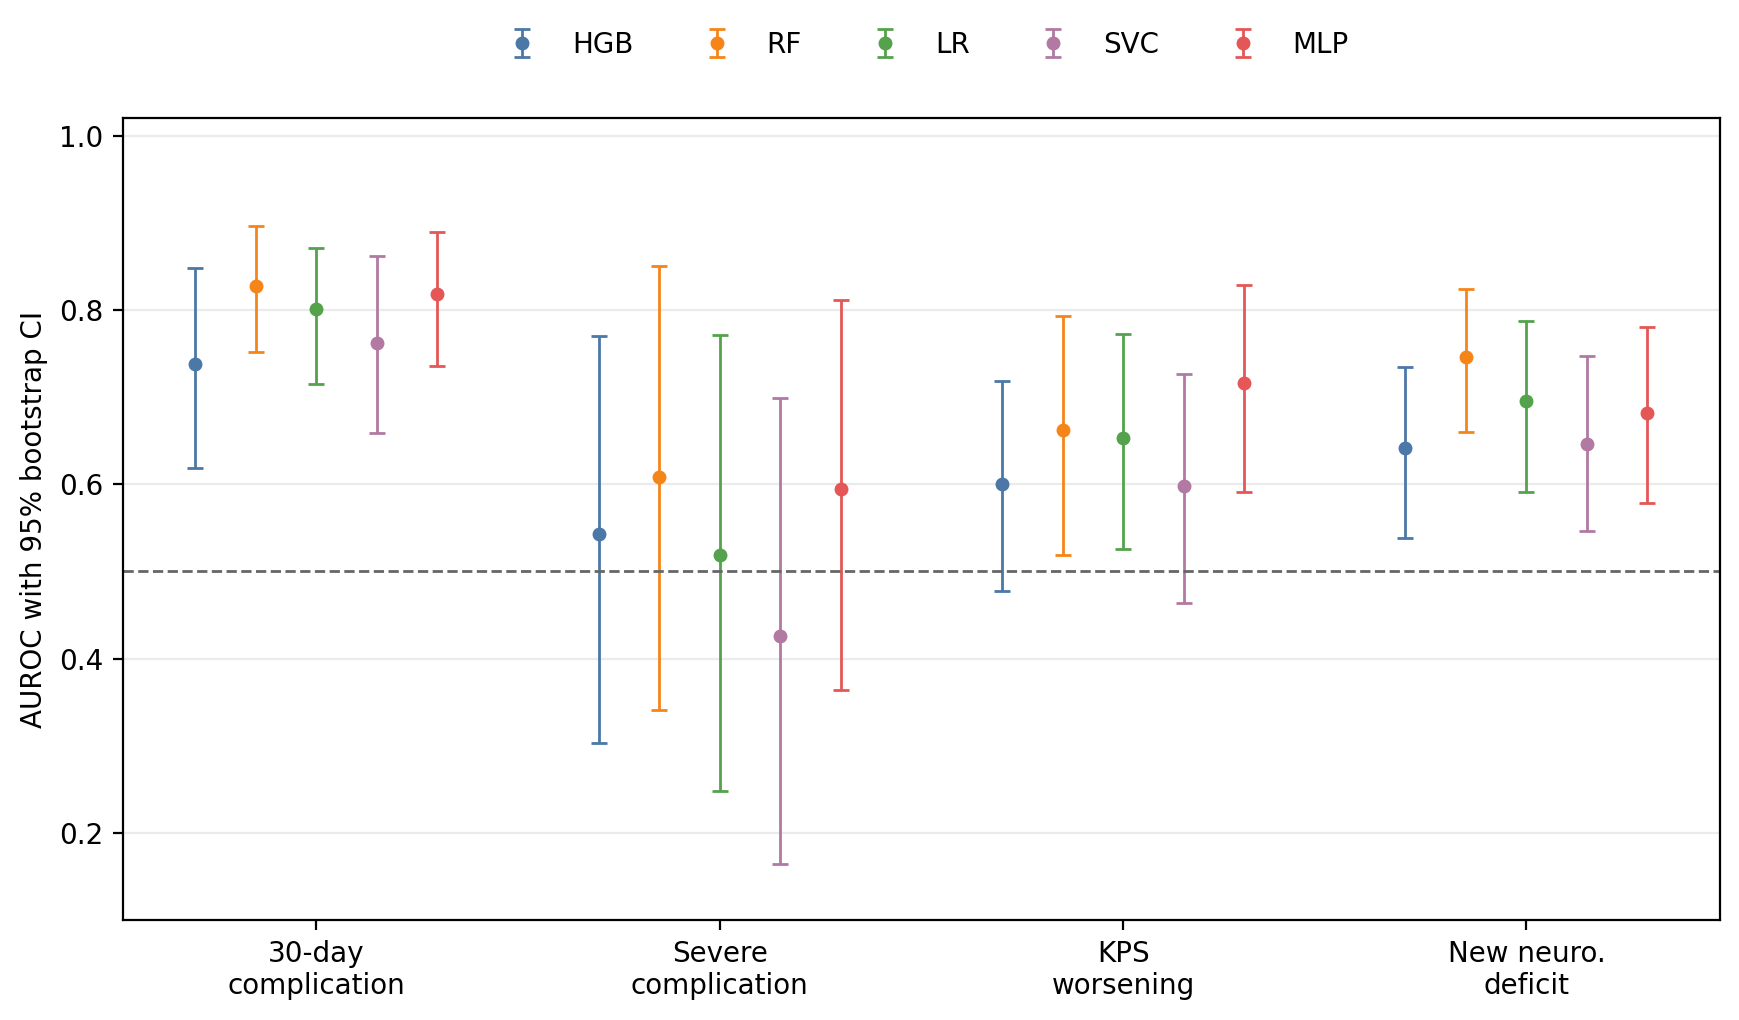
\includegraphics[width=0.95\linewidth]{figures/summary_auroc_ci.png}
\caption{AUROC with 95\% bootstrap confidence intervals for all full preoperative models. The dashed horizontal line indicates random discrimination, AUROC = 0.5. Severe-complication estimates have wide intervals because only 8 positive events were present in the temporal test set.}
\label{fig:summary-auroc}
\end{figure}

\begingroup
\small
\setlength{\tabcolsep}{5pt}
\begin{longtable}{p{3.0cm}p{1.4cm}p{3.6cm}p{1.3cm}p{3.6cm}}
\caption{Full preoperative discrimination on the final temporal test set. AP = average precision. AUROC and AP intervals are bootstrap 95\% confidence intervals.}\label{tab:full-performance}\\
\toprule
\shortstack[l]{Endpoint} & Model & AUROC (95\% CI) & p-value & AP (95\% CI) \\
\midrule
\endfirsthead
\toprule
\shortstack[l]{Endpoint} & Model & AUROC (95\% CI) & p-value & AP (95\% CI) \\
\midrule
\endhead
Complication 30d & HGB & 0.738 (0.619-0.848) & $<0.001$ & 0.284 (0.159-0.501) \\
Complication 30d & RF & 0.827 (0.752-0.896) & $<0.001$ & 0.328 (0.208-0.534) \\
Complication 30d & LR & 0.801 (0.715-0.872) & $<0.001$ & 0.298 (0.182-0.498) \\
Complication 30d & SVC & 0.762 (0.658-0.862) & 0.001 & 0.330 (0.180-0.557) \\
Complication 30d & MLP & 0.818 (0.735-0.889) & $<0.001$ & 0.315 (0.197-0.515) \\
\addlinespace
\shortstack[l]{Severe\\Complication} & HGB & 0.543 (0.303-0.770) & 0.340 & 0.082 (0.030-0.253) \\
\shortstack[l]{Severe\\Complication} & RF & 0.609 (0.341-0.850) & 0.150 & 0.131 (0.040-0.398) \\
\shortstack[l]{Severe\\Complication} & LR & 0.519 (0.248-0.771) & 0.435 & 0.090 (0.031-0.274) \\
\shortstack[l]{Severe\\Complication} & SVC & 0.426 (0.164-0.699) & 0.765 & 0.115 (0.023-0.398) \\
\shortstack[l]{Severe\\Complication} & MLP & 0.594 (0.364-0.812) & 0.191 & 0.096 (0.036-0.294) \\
\addlinespace
KPS worsened & HGB & 0.600 (0.478-0.719) & 0.064 & 0.214 (0.129-0.372) \\
KPS worsened & RF & 0.662 (0.519-0.793) & 0.006 & 0.316 (0.185-0.512) \\
KPS worsened & LR & 0.653 (0.526-0.772) & 0.008 & 0.273 (0.163-0.466) \\
KPS worsened & SVC & 0.598 (0.463-0.727) & 0.074 & 0.313 (0.160-0.494) \\
KPS worsened & MLP & 0.717 (0.591-0.829) & 0.001 & 0.326 (0.199-0.535) \\
\addlinespace
NND & HGB & 0.642 (0.538-0.735) & 0.006 & 0.385 (0.273-0.556) \\
NND & RF & 0.746 (0.660-0.824) & $<0.001$ & 0.440 (0.323-0.609) \\
NND & LR & 0.696 (0.591-0.787) & $<0.001$ & 0.454 (0.323-0.630) \\
NND & SVC & 0.647 (0.546-0.747) & 0.004 & 0.432 (0.292-0.582) \\
NND & MLP & 0.682 (0.579-0.780) & $<0.001$ & 0.464 (0.321-0.639) \\
\bottomrule
\end{longtable}
\endgroup

\begingroup
\small
\setlength{\tabcolsep}{4pt}
\begin{longtable}{p{3.0cm}p{1.4cm}rrrrrp{2.4cm}}
\caption{Threshold-dependent full preoperative performance on the final temporal test set. PPV = positive predictive value; NPV = negative predictive value.}\label{tab:full-threshold-performance}\\
\toprule
\shortstack[l]{Endpoint} & Model & Sens. & Spec. & PPV & NPV & Acc. & \shortstack{TN/FP/\\FN/TP} \\
\midrule
\endfirsthead
\toprule
\shortstack[l]{Endpoint} & Model & Sens. & Spec. & PPV & NPV & Acc. & \shortstack{TN/FP/\\FN/TP} \\
\midrule
\endhead
Complication 30d & HGB & 0.842 & 0.409 & 0.176 & 0.945 & 0.466 & 52/75/3/16 \\
Complication 30d & RF & 0.737 & 0.701 & 0.269 & 0.947 & 0.705 & 89/38/5/14 \\
Complication 30d & LR & 1.000 & 0.370 & 0.192 & 1.000 & 0.452 & 47/80/0/19 \\
Complication 30d & SVC & 1.000 & 0.039 & 0.135 & 1.000 & 0.164 & 5/122/0/19 \\
Complication 30d & MLP & 0.947 & 0.528 & 0.231 & 0.985 & 0.582 & 67/60/1/18 \\
\addlinespace
\shortstack[l]{Severe\\Complication} & HGB & 0.750 & 0.101 & 0.046 & 0.875 & 0.137 & 14/124/2/6 \\
\shortstack[l]{Severe\\Complication} & RF & 0.625 & 0.420 & 0.059 & 0.951 & 0.432 & 58/80/3/5 \\
\shortstack[l]{Severe\\Complication} & LR & 0.750 & 0.232 & 0.054 & 0.941 & 0.260 & 32/106/2/6 \\
\shortstack[l]{Severe\\Complication} & SVC & 1.000 & 0.000 & 0.055 & NA & 0.055 & 0/138/0/8 \\
\shortstack[l]{Severe\\Complication} & MLP & 0.750 & 0.283 & 0.057 & 0.951 & 0.308 & 39/99/2/6 \\
\addlinespace
KPS worsened & HGB & 0.957 & 0.138 & 0.172 & 0.944 & 0.267 & 17/106/1/22 \\
KPS worsened & RF & 0.783 & 0.512 & 0.231 & 0.926 & 0.555 & 63/60/5/18 \\
KPS worsened & LR & 0.913 & 0.260 & 0.188 & 0.941 & 0.363 & 32/91/2/21 \\
KPS worsened & SVC & 0.783 & 0.333 & 0.180 & 0.891 & 0.404 & 41/82/5/18 \\
KPS worsened & MLP & 0.913 & 0.195 & 0.175 & 0.923 & 0.308 & 24/99/2/21 \\
\addlinespace
NND & HGB & 0.974 & 0.194 & 0.298 & 0.955 & 0.397 & 21/87/1/37 \\
NND & RF & 0.974 & 0.361 & 0.349 & 0.975 & 0.521 & 39/69/1/37 \\
NND & LR & 0.921 & 0.287 & 0.313 & 0.912 & 0.452 & 31/77/3/35 \\
NND & SVC & 0.842 & 0.361 & 0.317 & 0.867 & 0.486 & 39/69/6/32 \\
NND & MLP & 0.816 & 0.389 & 0.320 & 0.857 & 0.500 & 42/66/7/31 \\
\bottomrule
\end{longtable}
\endgroup

The benchmark indicates that the models did not behave uniformly across outcomes, which is expected because the endpoints differ in event frequency and clinical definition. As shown in Table~\ref{tab:full-performance}, RF achieved the highest AUROC for Complication 30d and, according to Table~\ref{tab:full-threshold-performance}, a more balanced sensitivity-specificity profile than LR, SVC, or MLP. LR and SVC reached very high sensitivity for this endpoint, but this came with many false positives, which would reduce usefulness if the prediction were used to trigger additional review or intervention. For Severe Complication, the AUROC estimates were uncertain and the p values did not provide strong evidence of discrimination. This result should not be interpreted as proof that the endpoint is unpredictable; it mainly reflects the very small number of severe events in the temporal test set. For KPS worsened, MLP achieved the highest AUROC, but specificity remained low at the selected recall-oriented threshold, so a deployment focused on this endpoint would require careful threshold calibration. For NND, RF produced the strongest AUROC and high sensitivity, suggesting that the model may be most useful as a screening tool. Overall, the results support a recall-sensitive use case, but they also show that decision thresholds should be chosen according to the clinical cost of false positives and false negatives rather than copied automatically from the benchmark.

\section{Feature importance and reduced-feature experiments}

We used permutation feature importance to estimate how much each original input variable contributes to prediction \cite{fisher2019modelreliance}. After training a model, we evaluated it on the test set, then repeated the evaluation after randomly shuffling one feature across patients. Shuffling destroys the relationship between that feature and the outcome while preserving the marginal distribution of that feature. If model performance decreases substantially after shuffling, we considered the feature important for that fitted model.

We computed permutation importance with scikit-learn \code{permutation_importance}, five repeats, and \code{random_state=42}. For scikit-learn binary classifiers that expose predicted probabilities, we used AUROC as the scoring metric. For Torch models, our implementation falls back to accuracy scoring because Torch classifiers were not included in the AUROC scoring branch. We therefore considered this distinction when comparing feature-importance magnitudes between Torch and non-Torch models.

We used feature importance for two roles: interpretation, because it identifies variables that the fitted model relied on most for held-out prediction, and feature reduction, because it supports reducing the number of required inputs in the doctor-facing application. Reducing the number of variables is clinically necessary because a model requiring many manual fields can be burdensome and less likely to be used. It may also reduce redundancy when several variables carry overlapping information. Permutation importance is not causal inference; it identifies predictive contribution for a fitted model, not independent causal effect.

Figure~\ref{fig:feature-importance} shows the permutation-importance profiles for the best full model by AUROC for each endpoint. Table~\ref{tab:fi} reports the same analysis numerically for the five highest-ranked variables, so that the visual ranking is accompanied by exact mean importance, variability across repeats, and exploratory p values.

\begin{figure}[H]
\centering
\begin{subfigure}{0.48\linewidth}
\centering
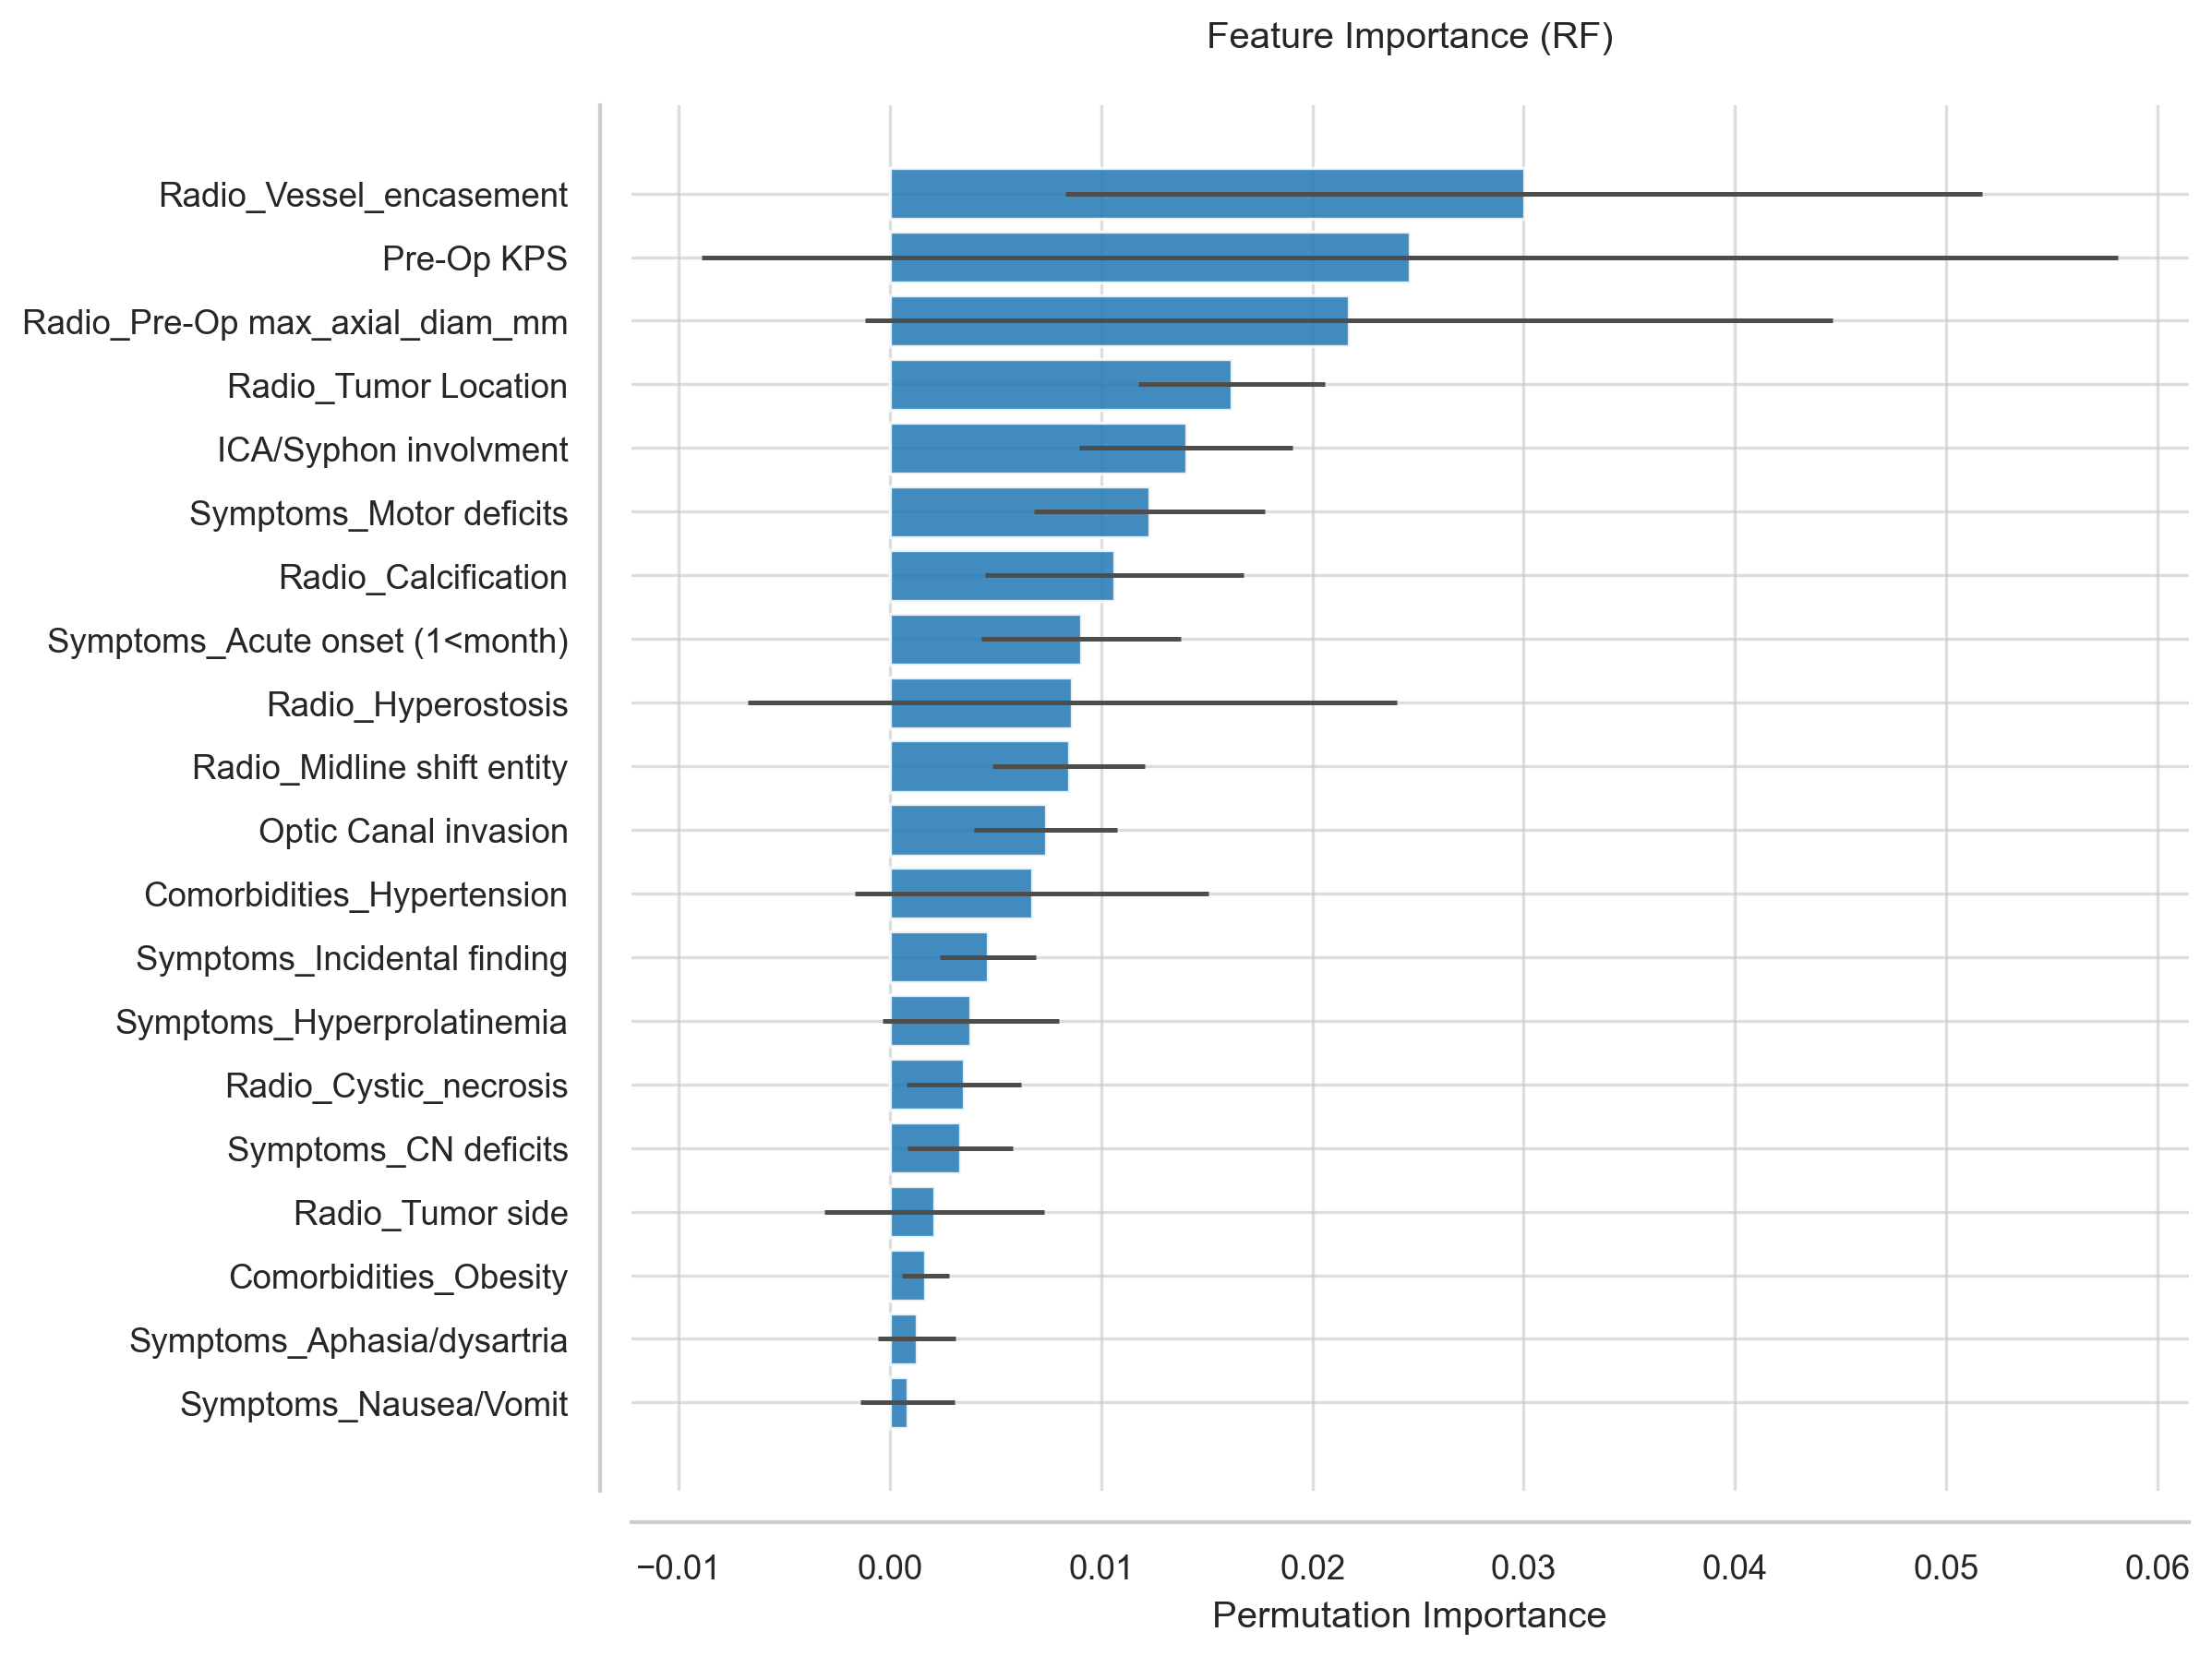
\includegraphics[width=\linewidth]{figures/fi_complications30d_rf.png}
\caption{Complication 30d, RF}
\end{subfigure}
\hfill
\begin{subfigure}{0.48\linewidth}
\centering
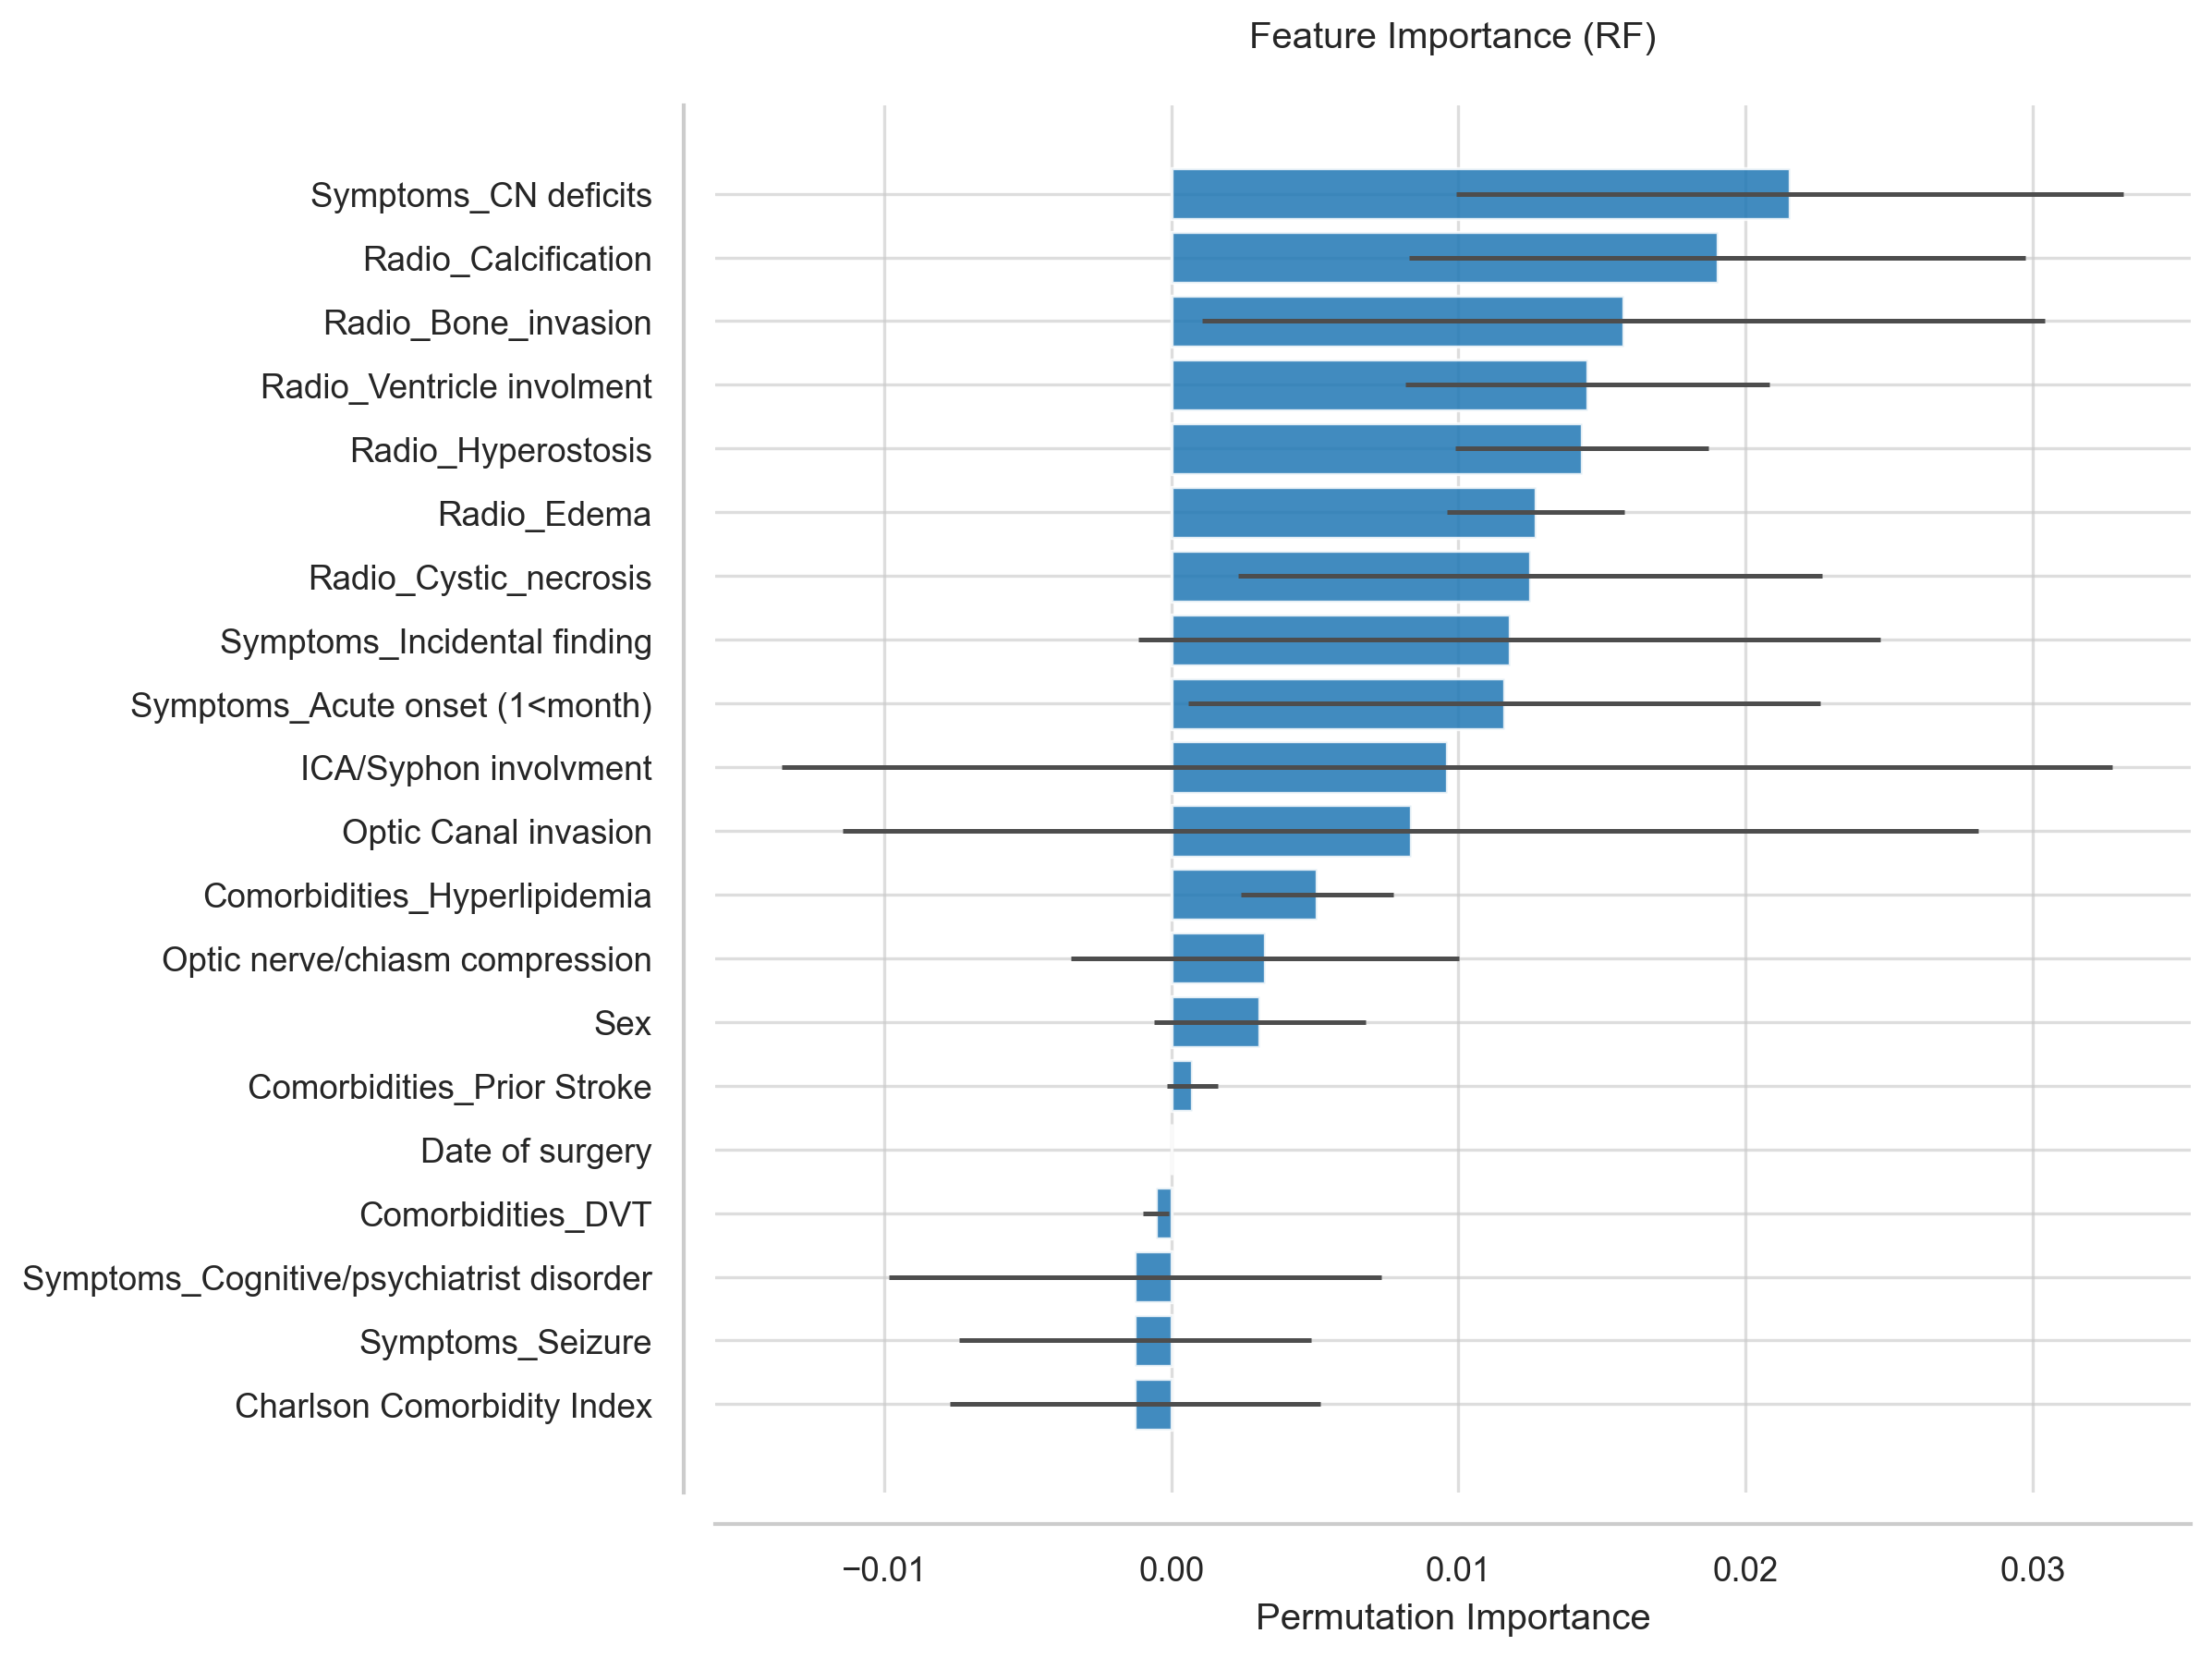
\includegraphics[width=\linewidth]{figures/fi_severe_rf.png}
\caption{Severe Complication, RF}
\end{subfigure}

\vspace{0.3cm}
\begin{subfigure}{0.48\linewidth}
\centering
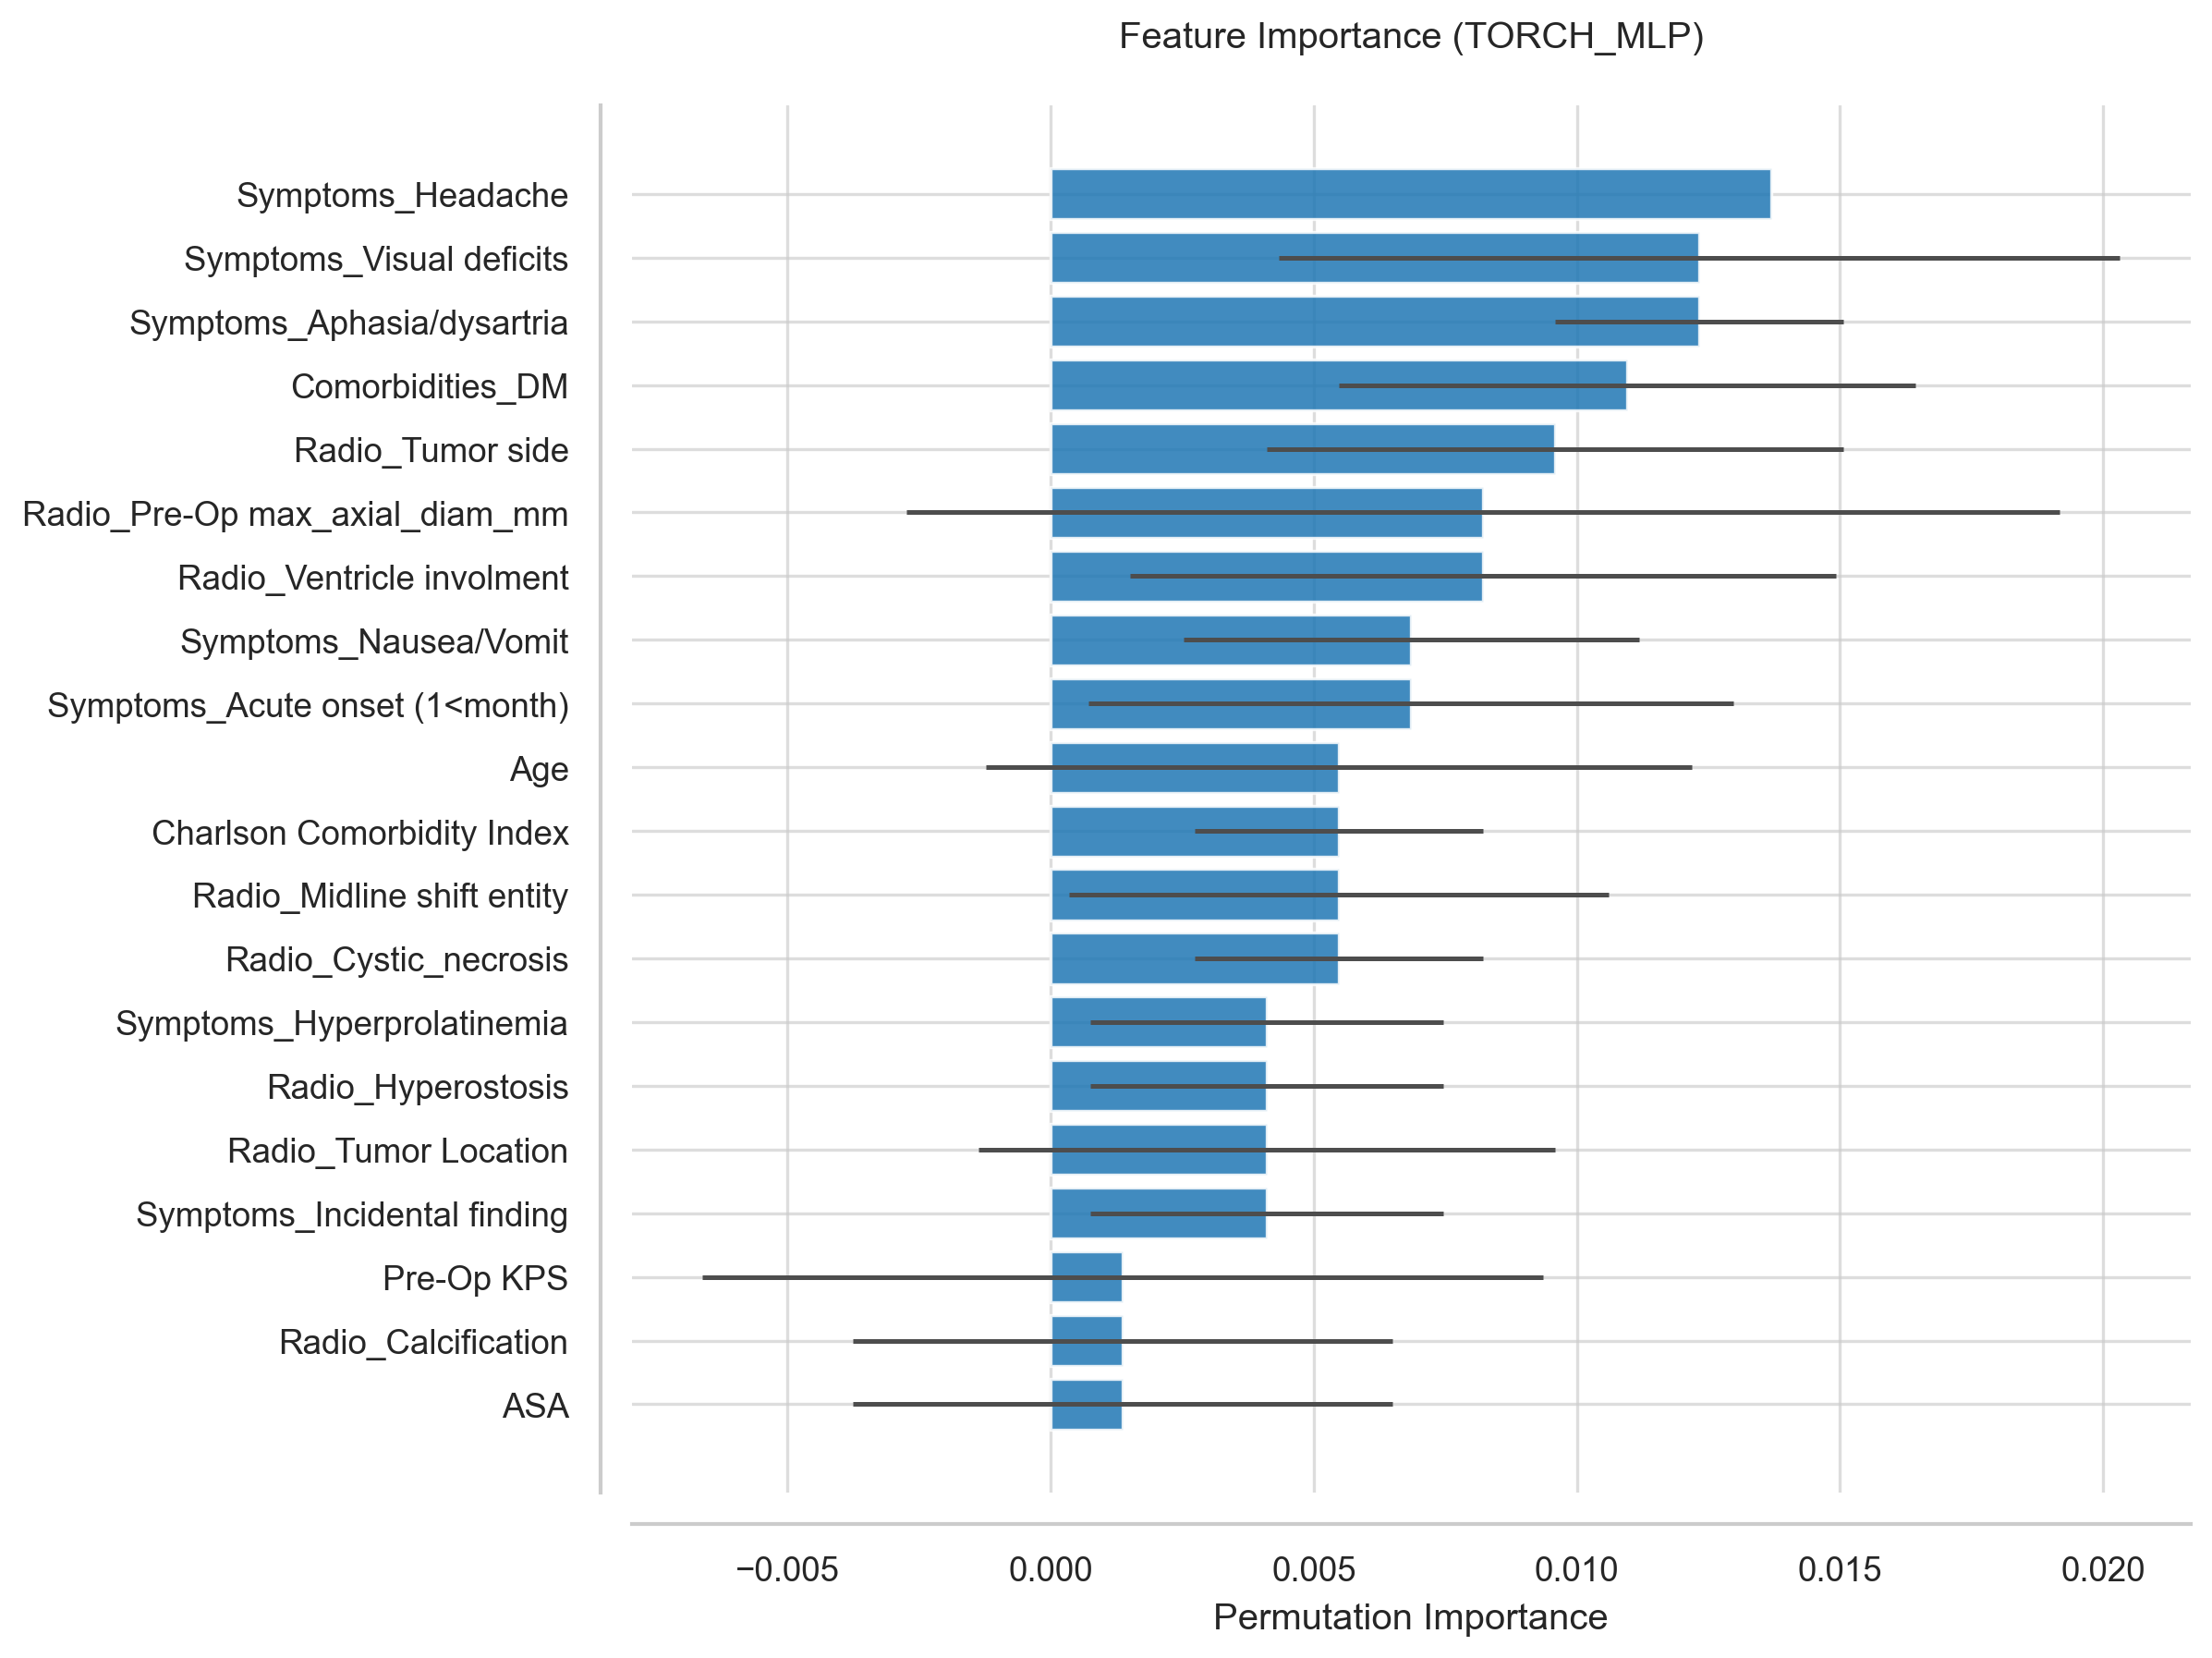
\includegraphics[width=\linewidth]{figures/fi_kps_torch_mlp.png}
\caption{KPS worsened, MLP}
\end{subfigure}
\hfill
\begin{subfigure}{0.48\linewidth}
\centering
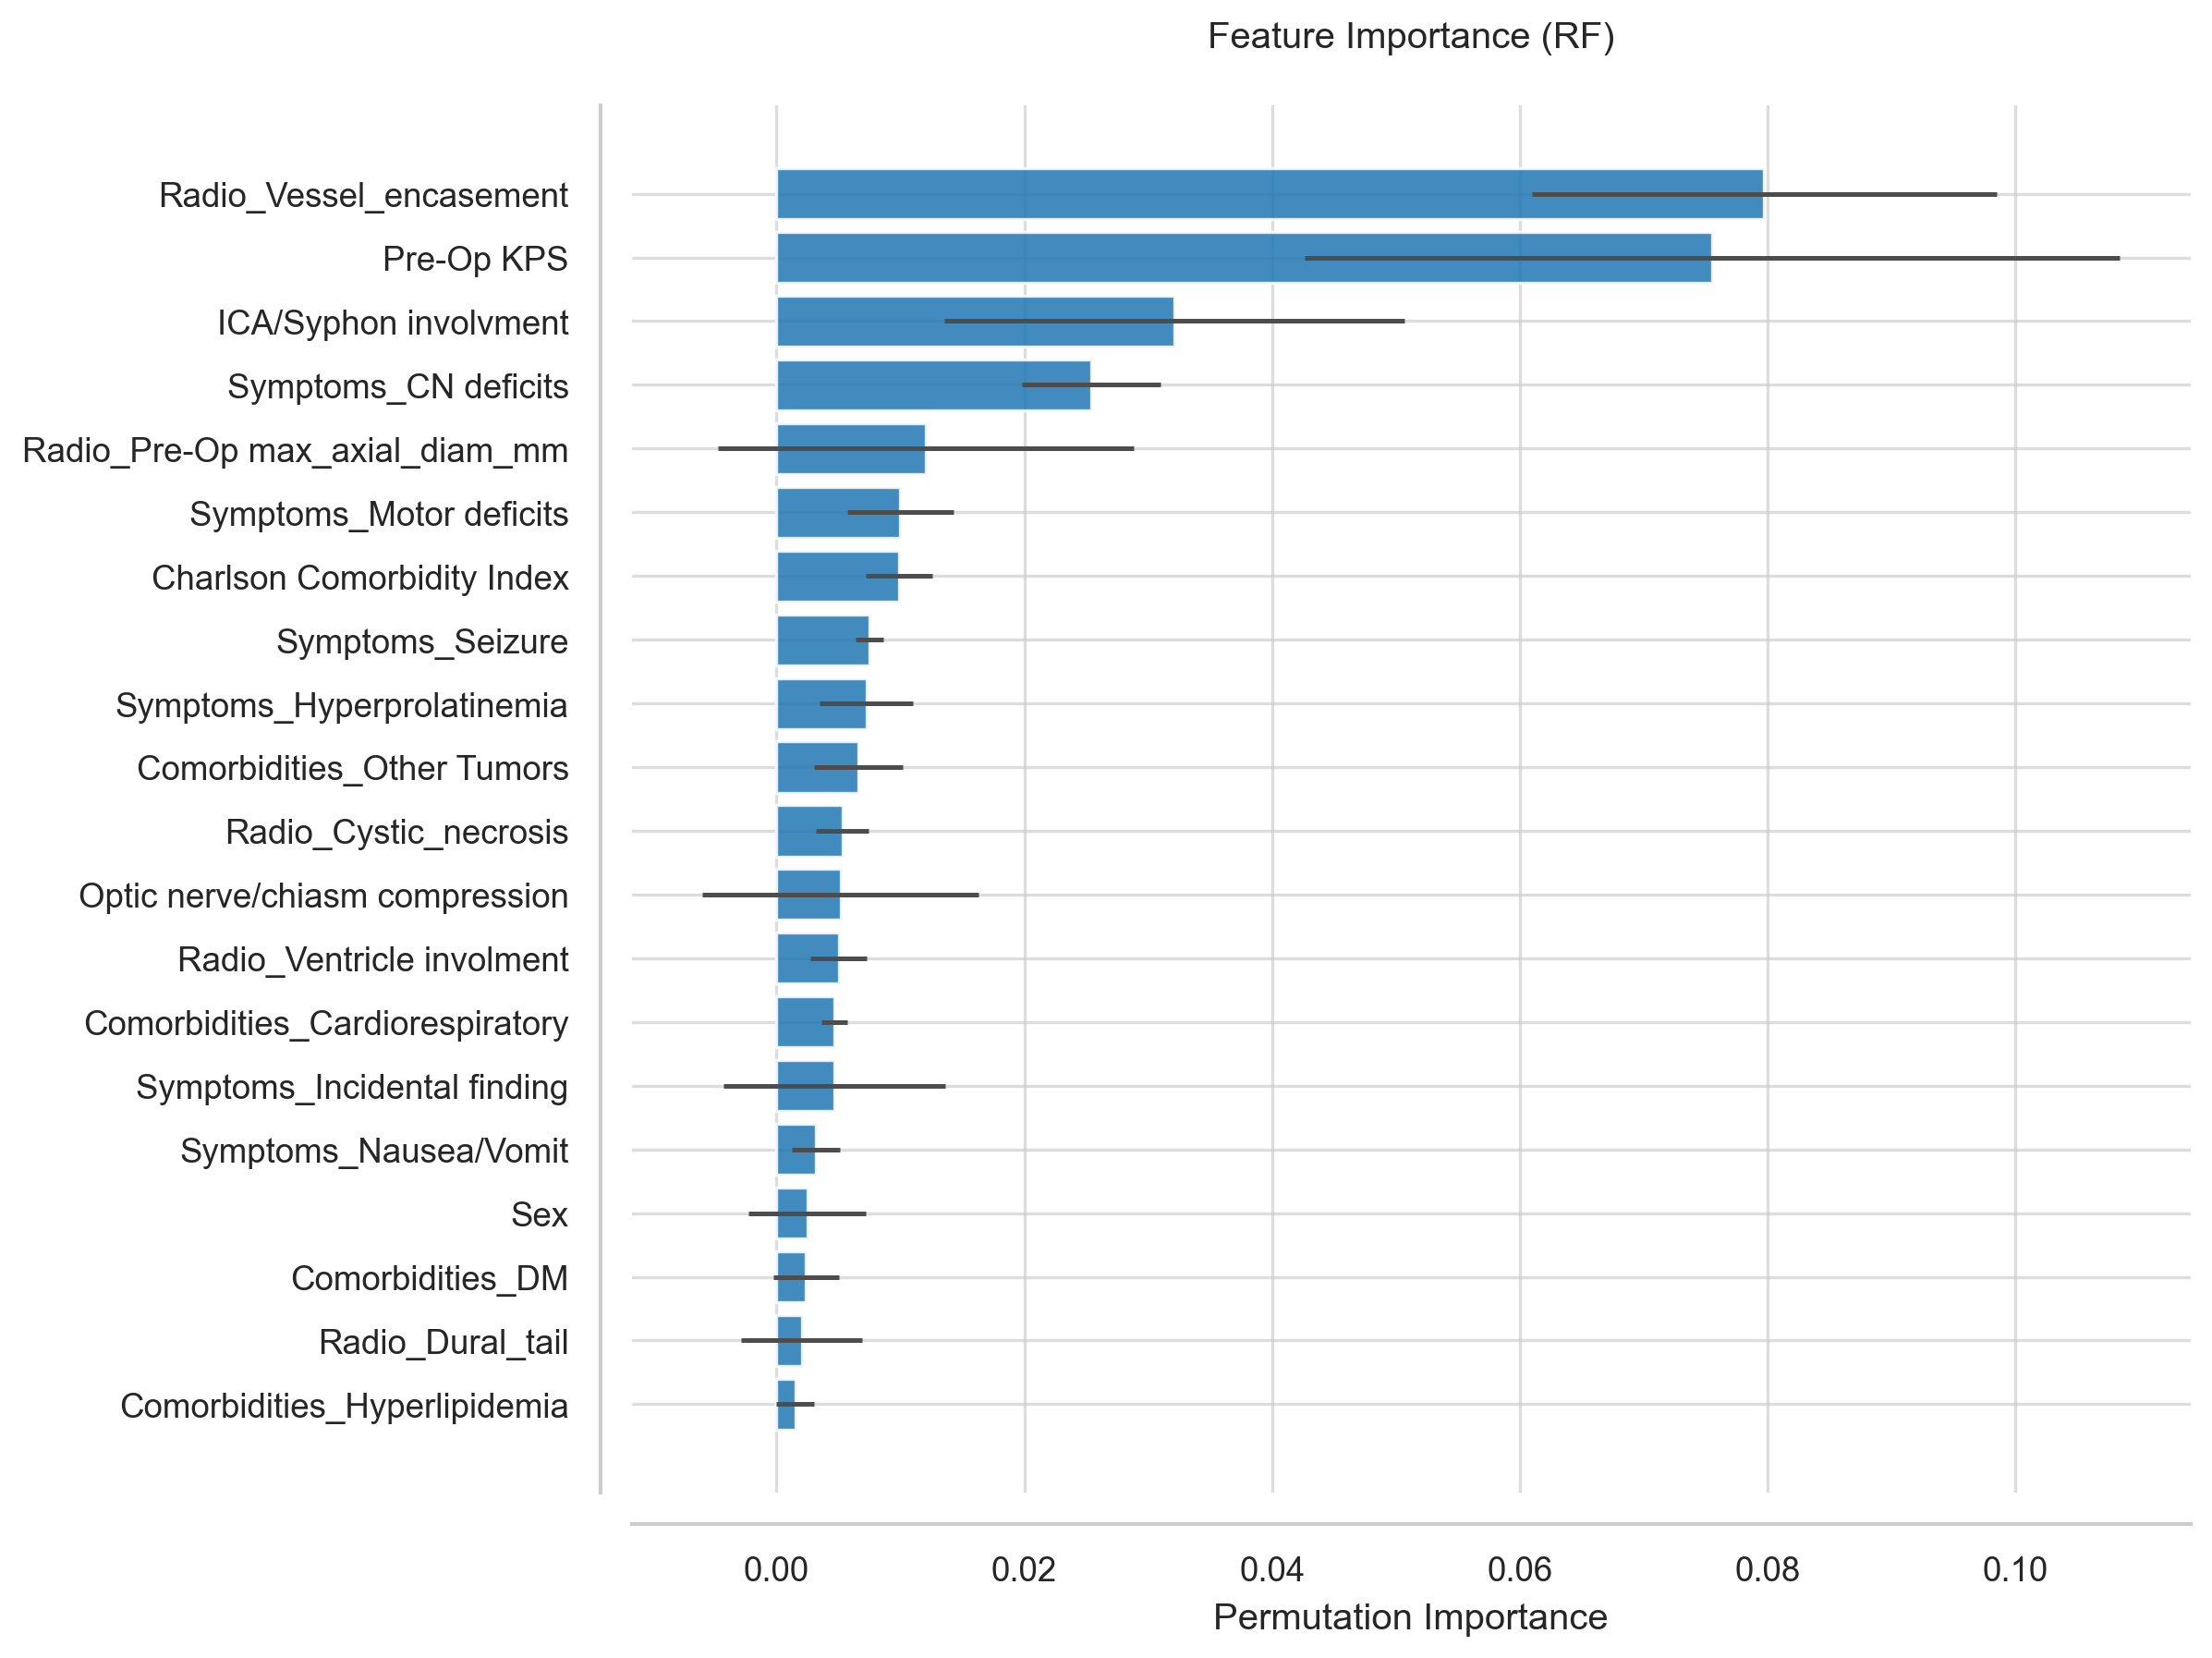
\includegraphics[width=\linewidth]{figures/fi_neuro_rf.png}
\caption{NND, RF}
\end{subfigure}
\caption{Permutation feature importance for the best full preoperative model by AUROC for each endpoint. Importance is the decrease in predictive score after random permutation of a single predictor. Larger decreases indicate greater dependence of the fitted model on that predictor.}
\label{fig:feature-importance}
\end{figure}

\begingroup
\scriptsize
\setlength{\tabcolsep}{3pt}
\begin{longtable}{p{2.1cm}p{1.0cm}rp{6.3cm}rrr}
\caption{Top permutation-importance features for the best full model by AUROC for each endpoint. Approximate p values are exploratory and are computed from five permutation repeats.}\label{tab:fi}\\
\toprule
\shortstack[l]{Endpoint} & Model & Rank & Feature & Mean & SD & \shortstack{Approx.\\p} \\
\midrule
\endfirsthead
\toprule
\shortstack[l]{Endpoint} & Model & Rank & Feature & Mean & SD & \shortstack{Approx.\\p} \\
\midrule
\endhead
Complication 30d & RF & 1 & Vessel encasement & 0.030 & 0.022 & 0.018 \\
Complication 30d & RF & 2 & Preoperative KPS & 0.025 & 0.034 & 0.088 \\
Complication 30d & RF & 3 & Max axial tumor diameter & 0.022 & 0.023 & 0.051 \\
Complication 30d & RF & 4 & Tumor location & 0.016 & 0.004 & 0.001 \\
Complication 30d & RF & 5 & ICA/Syphon involvement & 0.014 & 0.005 & 0.002 \\
\addlinespace
\shortstack[l]{Severe\\Complication} & RF & 1 & Cranial nerve deficits & 0.022 & 0.012 & 0.007 \\
\shortstack[l]{Severe\\Complication} & RF & 2 & Calcification & 0.019 & 0.011 & 0.008 \\
\shortstack[l]{Severe\\Complication} & RF & 3 & Bone invasion & 0.016 & 0.015 & 0.037 \\
\shortstack[l]{Severe\\Complication} & RF & 4 & Ventricle involvement & 0.014 & 0.006 & 0.003 \\
\shortstack[l]{Severe\\Complication} & RF & 5 & Hyperostosis & 0.014 & 0.004 & 0.001 \\
\addlinespace
KPS worsened & MLP & 1 & Headache & 0.014 & 0.000 & $<$0.001 \\
KPS worsened & MLP & 2 & Visual deficits & 0.012 & 0.008 & 0.013 \\
KPS worsened & MLP & 3 & Aphasia/dysarthria & 0.012 & 0.003 & $<$0.001 \\
KPS worsened & MLP & 4 & Diabetes mellitus & 0.011 & 0.005 & 0.006 \\
KPS worsened & MLP & 5 & Tumor side & 0.010 & 0.005 & 0.009 \\
\addlinespace
NND & RF & 1 & Vessel encasement & 0.080 & 0.019 & $<$0.001 \\
NND & RF & 2 & Preoperative KPS & 0.076 & 0.033 & 0.003 \\
NND & RF & 3 & ICA/Syphon involvement & 0.032 & 0.019 & 0.009 \\
NND & RF & 4 & Cranial nerve deficits & 0.025 & 0.006 & $<$0.001 \\
NND & RF & 5 & Max axial tumor diameter & 0.012 & 0.017 & 0.091 \\
\bottomrule
\end{longtable}
\endgroup

The feature-importance patterns in Figure~\ref{fig:feature-importance} and Table~\ref{tab:fi} suggest that anatomical complexity and baseline neurological reserve were recurrent contributors. Vessel encasement, preoperative KPS, tumor diameter, ICA/Syphon involvement, cranial nerve deficits, and tumor location appeared among the most relevant variables across endpoints. Severe-complication importance rankings should be interpreted cautiously because the test set contained only 8 positive cases. For KPS worsened, the best model was the multilayer perceptron, and its feature-importance values were computed using accuracy rather than AUROC; these rankings are therefore supportive rather than definitive.

\subsection{Reduced-feature performance}

We designed the reduced-feature experiments to address a practical deployment problem. The full preoperative configuration has 40 input variables. Some of these variables may be redundant, unavailable in some centers, or too burdensome for routine manual entry. A reduced model can be more usable if it preserves most of the full model's discrimination while requiring fewer fields.

Each saved reduced-feature experiment uses 30 predictors. We used the same temporal split and selected hyperparameters. Figure~\ref{fig:full-reduced-summary} summarizes the mean AUROC across models for the full and reduced feature sets, and Table~\ref{tab:reduced} reports the corresponding model-level deltas. Black diamonds in the figure indicate the best model within each feature set.

\begin{figure}[H]
\centering
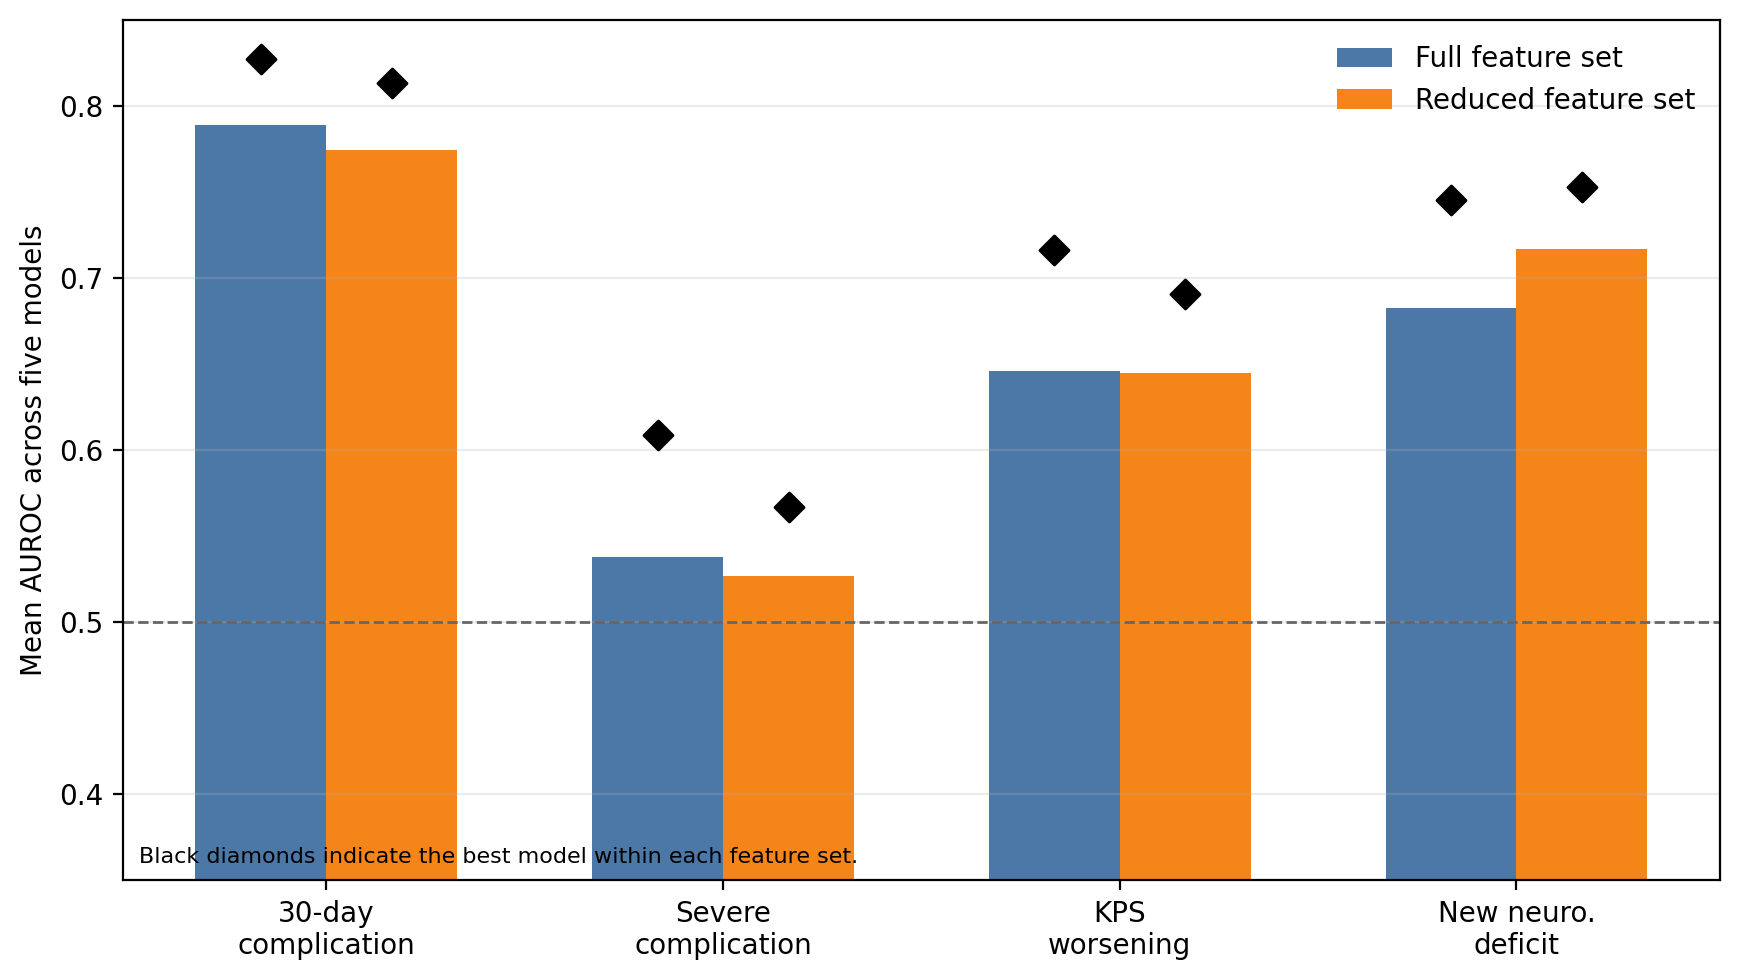
\includegraphics[width=0.95\linewidth]{figures/summary_full_vs_reduced_auroc.png}
\caption{Mean AUROC across the five evaluated models for the full 40-feature set and the reduced 30-feature set. Black diamonds show the best model within each feature set.}
\label{fig:full-reduced-summary}
\end{figure}

\begingroup
\scriptsize
\setlength{\tabcolsep}{3pt}
\begin{longtable}{p{2.0cm}p{1.0cm}rrrrrr}
\caption{Full versus reduced feature performance. Delta values are reduced minus full. Positive delta values favor the reduced-feature model. AP = average precision.}\label{tab:reduced}\\
\toprule
\shortstack[l]{Endpoint} & Model & \shortstack{Full\\features} & \shortstack{Reduced\\features} & \shortstack{AUROC\\full} & \shortstack{AUROC\\reduced} & \shortstack{Delta\\AUROC} & \shortstack{Delta\\AP} \\
\midrule
\endfirsthead
\toprule
\shortstack[l]{Endpoint} & Model & \shortstack{Full\\features} & \shortstack{Reduced\\features} & \shortstack{AUROC\\full} & \shortstack{AUROC\\reduced} & \shortstack{Delta\\AUROC} & \shortstack{Delta\\AP} \\
\midrule
\endhead
Complication 30d & HGB & 40 & 30 & 0.738 & 0.706 & -0.032 & -0.060 \\
Complication 30d & RF & 40 & 30 & 0.827 & 0.811 & -0.017 & -0.034 \\
Complication 30d & LR & 40 & 30 & 0.801 & 0.798 & -0.002 & -0.014 \\
Complication 30d & SVC & 40 & 30 & 0.762 & 0.744 & -0.018 & -0.023 \\
Complication 30d & MLP & 40 & 30 & 0.818 & 0.814 & -0.005 & -0.006 \\
\addlinespace
\shortstack[l]{Severe\\Complication} & HGB & 40 & 30 & 0.543 & 0.548 & 0.005 & 0.047 \\
\shortstack[l]{Severe\\Complication} & RF & 40 & 30 & 0.609 & 0.517 & -0.091 & -0.003 \\
\shortstack[l]{Severe\\Complication} & LR & 40 & 30 & 0.519 & 0.567 & 0.048 & 0.027 \\
\shortstack[l]{Severe\\Complication} & SVC & 40 & 30 & 0.426 & 0.450 & 0.024 & -0.028 \\
\shortstack[l]{Severe\\Complication} & MLP & 40 & 30 & 0.594 & 0.551 & -0.043 & 0.034 \\
\addlinespace
KPS worsened & HGB & 40 & 30 & 0.600 & 0.613 & 0.013 & 0.043 \\
KPS worsened & RF & 40 & 30 & 0.662 & 0.691 & 0.029 & 0.037 \\
KPS worsened & LR & 40 & 30 & 0.653 & 0.651 & -0.002 & -0.010 \\
KPS worsened & SVC & 40 & 30 & 0.598 & 0.622 & 0.024 & -0.015 \\
KPS worsened & MLP & 40 & 30 & 0.717 & 0.645 & -0.071 & -0.066 \\
\addlinespace
NND & HGB & 40 & 30 & 0.642 & 0.732 & 0.090 & 0.127 \\
NND & RF & 40 & 30 & 0.746 & 0.753 & 0.007 & 0.051 \\
NND & LR & 40 & 30 & 0.696 & 0.709 & 0.013 & 0.017 \\
NND & SVC & 40 & 30 & 0.647 & 0.681 & 0.035 & 0.008 \\
NND & MLP & 40 & 30 & 0.682 & 0.709 & 0.028 & 0.092 \\
\bottomrule
\end{longtable}
\endgroup

The reduced-feature experiments in Figure~\ref{fig:full-reduced-summary} and Table~\ref{tab:reduced} do not show a uniform loss of performance. For 30-day complications, the reduced models show only small AUROC decreases for random forest, logistic regression, support vector classifier, and multilayer perceptron. For KPS worsening, random forest and support vector classifier improve slightly under the reduced set, while the multilayer perceptron decreases. For new neurological deficits, all reduced models improve in AUROC relative to the full-feature counterparts, suggesting that removing some variables may reduce noise or redundancy for that endpoint. For severe complications, results remain unstable because the endpoint has very few positive test events.

These findings support further work toward a clinically feasible reduced-input tool. Because the reduced-feature selection rule was not specified as a fully independent experimental protocol before model evaluation, the reduced-feature results should be interpreted as exploratory rather than as a definitive feature-selection procedure.

\section{Software implementation and user interfaces}

We implemented two Flask-based interfaces to connect the statistical workflow to practical use. The physician-facing interface is a clinical risk-assessment tool. It presents available prediction configurations, builds a patient-entry form from the required variables, and groups the fields into clinically meaningful sections such as demographics, functional status, comorbidities, symptoms, imaging findings, vascular involvement, and cranial-nerve or brainstem involvement. The intended clinical workflow assumes that the physician completes all required fields before prediction. For each endpoint, the interface returns the estimated risk probability, the model used, the trained decision threshold, and a qualitative risk category based on configurable low and high risk boundaries. The interface also includes a notice that the output is decision support and must be interpreted with the full clinical picture.

The technician-facing interface is designed for maintenance and model updating rather than patient-level use. It allows a technical operator to select endpoints, choose model families, define or revise the feature subset, adjust training parameters, and launch new training runs. It also provides progress monitoring during training and a results explorer for completed experiments. The results view summarizes performance metrics, ROC and precision-recall curves, confusion matrices, model-comparison plots, and permutation-importance outputs. This makes the interface useful for iterative feature reduction: the technician can train a candidate reduced model, inspect performance and feature importance, adjust the feature set, and repeat the process.

The two-interface design separates clinical use from technical maintenance. Clinicians interact with a constrained prediction interface, whereas technical users can retrain, monitor, and update the system. This separation reduces the risk that clinical users accidentally modify model settings while still allowing the software to evolve as new data, revised feature sets, or updated decision thresholds become available.

\section{Limitations relevant to the technical methodology}

First, we performed internal temporal validation, not external validation. Temporal splitting is more realistic than random splitting, but all data still come from the same retrospective study dataset. External validation is required before clinical deployment.

Second, several endpoints are imbalanced. Severe complications are especially rare in the temporal test set, with only 8 positive events. Metrics for that endpoint have wide confidence intervals and should not be overinterpreted.

Third, the selected decision thresholds are tuned to favor recall. This may be appropriate for screening but causes low specificity and low positive predictive value for several models. The final threshold should be matched to the clinical use case. A tool designed to alert surgeons to possible risk may accept more false positives than a tool designed to allocate scarce postoperative resources.

Fourth, permutation feature importance depends on the fitted model, test set, scoring metric, and correlations among predictors. If two variables contain similar information, shuffling one may show limited importance because the other variable can partially substitute for it. Feature importance therefore identifies predictive contribution, not independent causal effect.

Fifth, the reduced-feature experiments are promising but not fully reproducible from an explicit selection rule in the current experimental protocol. They should therefore be interpreted as exploratory evidence for input reduction rather than as a definitive reduced-feature model specification.

\bibliographystyle{unsrt}
\bibliography{technical_methodology_references}

\end{document}
